\documentclass[../../layout.tex]{subfiles}

\begin{document}
\chapter{Modelagem do Hardware}
\hspace*{3em}A montagem e relação entre os dispositivos, microcontroladores e conexões pode ser resumida de acordo com a seguinte exemplificação: o microcomputador comunica ou com os sensores e dispositivos, sejam eles sensores de temperatura, humidade, luminosidade que captam valores do ambiente em que se localiza ou com lâmpadas ou leds e enviam para esse microcomputador, na qual é o próprio servidor em que armazena localmente suas informações recebidas e processa de forma organizada para otimizar seu uso. \par
\hspace*{3em}Esse microcomputador processa então essas informações para representar como interface humana para que o usuário possa integarir, através de um navegador da internet em outro aparelho qualquer, seja celular ou computador. Na Figura \ref{fig:hwmodel} é representado o diagrama de blocos do hardware deste projeto, onde está separada por 3 partes principais:

\begin{enumerate}[label=\alph*)]
\itemsep0em
    \item Fonte de alimentação; 
    \item Raspberry Pi 3 B+, o microcomputador do projeto;
    \item Sensores, responsáveis pela comunicação externa do microcomputador ao ambiente instalado.
\end{enumerate}
 
\begin{figure}[H]
\centering
\caption{Diagrama de \emph{Hardware}}
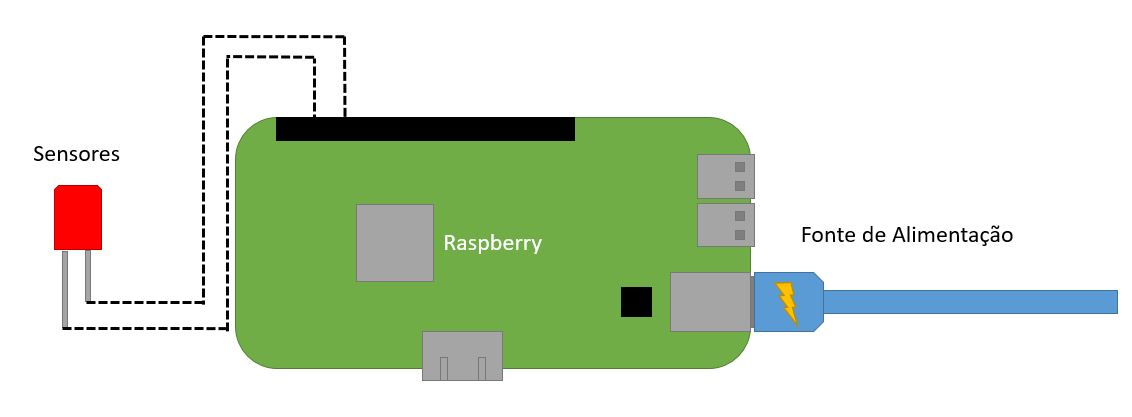
\includegraphics[width=0.5\textwidth]{assets/static/img/hwmodel.jpg}
\label{fig:hwmodel}

\begin{minipage}{0.5\textwidth}
\end{minipage}
\end{figure}

\hspace*{3em}Neste projeto foi escolhido o microcomputador Raspberry Pi 3 B+, exibido na Figura \ref{fig:rpi}, desenvolvido no final de 2014 pela \emph{Raspberry Pi Foundation} com as seguintes especificações:
\begin{enumerate}[label=\alph*)]
\itemsep0em
    \item SoC (\emph{System On a Chip}): Broadcom BCM2837B0 quad-core Cortex-A53 (ARMv8) 64-bit 1.4GHz;
    \item 1 entrada \emph{Gigabit Ethernet} e WiFi (2,4 e 5 GHz);
    \item memória: 1GB LPDDR2 SDRAM;
    \item GPIO (\emph{General Purpose Input/Output})de 40 pinos;
    \item Entrada de 5V/ 2,5A;
    \item memória: 1GB LPDDR2 SDRAM;
    \item armazenamento: cartão \emp{Micro SD}.
\end{enumerate}

\begin{figure}[H]
\centering
\caption{Raspberry Pi}
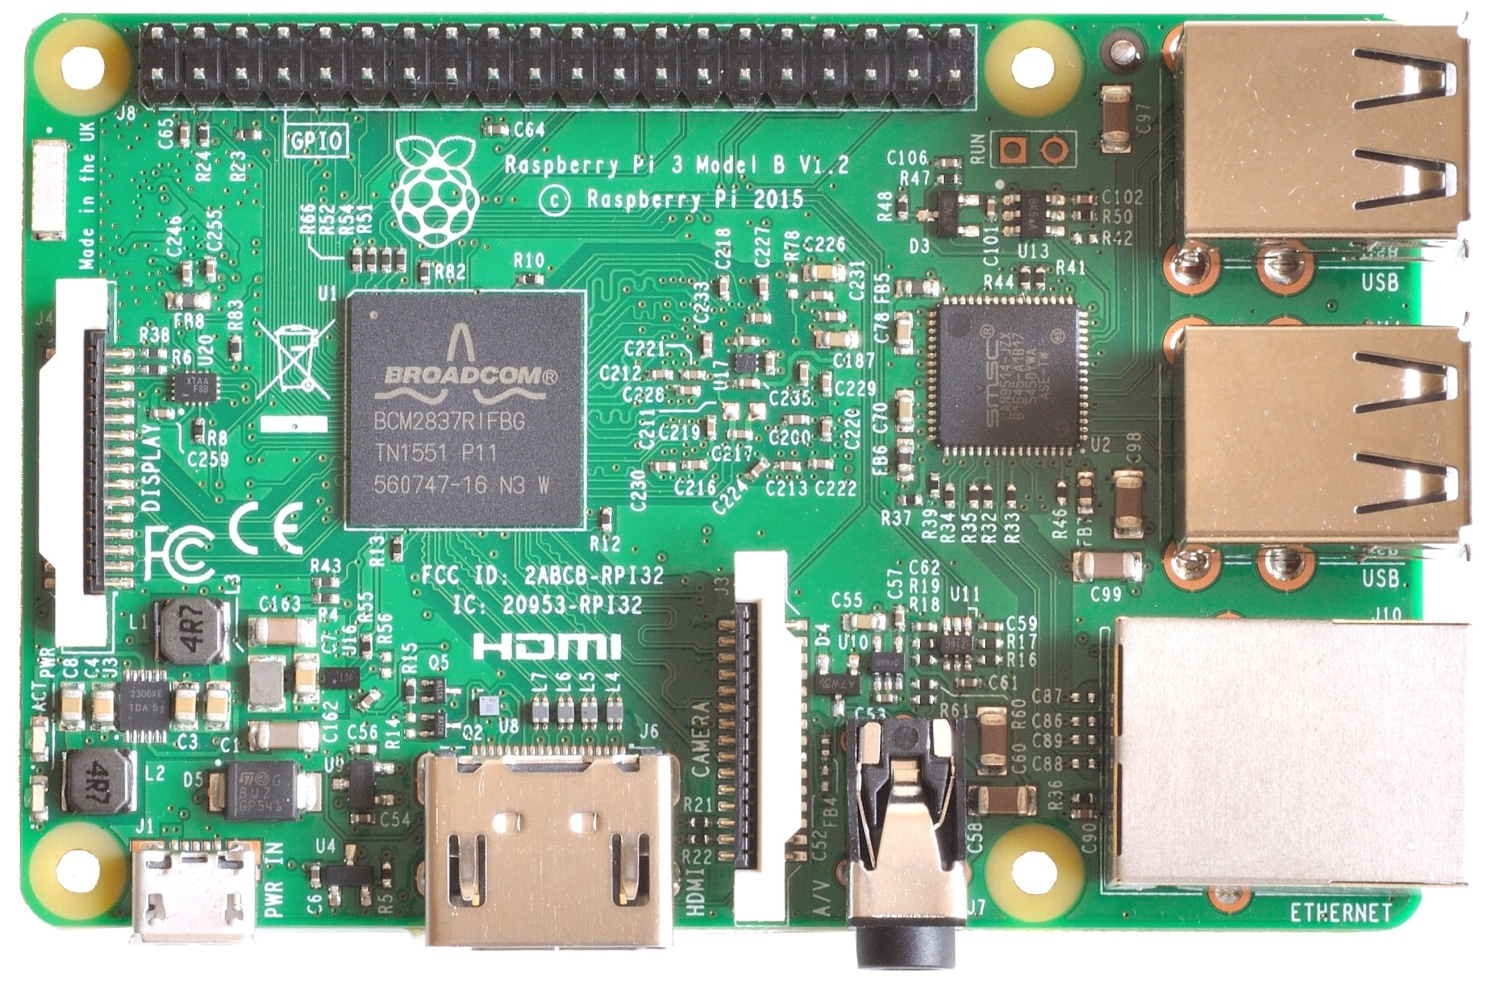
\includegraphics[width=0.5\textwidth]{assets/static/img/rpi.jpg}
\label{fig:rpi}

\begin{minipage}{0.5\textwidth}
\raggedright \footnotesize Fonte: Retirado de \acite{rpi}
\end{minipage}
\end{figure}

\hspace*{3em}O motivo deste microprocessador ser escolhido foi devido à praticidade de seu uso, seja informações na internet, quanto a portabilidade nas conexões de GPIO, conexão à internet via cabo ou WiFi, quantidade de memória suficiente para um sistema operacional ideal, baixo consumo de energia e preço agressivo comparado à outros modelos de processadores ou microprocessadores.

\section{Sensores}
\section{Conexão dos sensores à Raspberry Pi 3B+}
\hspace*{3em}Todas as conexões que realizamos dos sensores e leds foram feitas atráves da GPIO do microprocessador, o Raspberry, através de uma \emph{protoboard} e cabos para conectá-los.
\hspace*{3em}Sensores, atuadores, microcontroladores são componentes vastamente utilizados para projetos de Internet das Coisas para sua conectividade e interação sejam realizadas \cite{sensores_iot}. Sensores por sua vez, são práticos e de baixo custo para trazer um valor final ao projeto, como monitorar temperatura de uma sala de servidor, controlar humidade de um campo de plantações, abertura de cortinas, entre outros objetivos.
\subsection{Sensor de Luminosidade - BH1750}
\hspace*{3em}O sensor de luminosidade BH1750 \ref{fig:BH1750} é um dispositivo sensível à luz que possui uma interface de comunicação 16 \emph{bits} e interface de comunicação de acordo com o protocolo I2C e uma característica de sensibilidade ao espectro de luz muito parecido ao olho humano.
\hspace*{3em}O sensor BH1750 possui as seguintes especificações:
\begin{enumerate}[label=\alph*)]
\itemsep0em
    \item sensor de luminosidade com faixa de operação de 1 lux a 65.535 lux, precisão de +/- 1 lux e resolução de 1 lux.
\end{enumerate}

\begin{figure}[H]
\centering
\caption{Sensor de Luminosidade - BH1750}
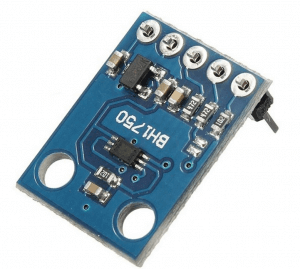
\includegraphics[width=0.5\textwidth]{assets/static/img/BH1750.jpg}
\label{fig:BH1750}

\begin{minipage}{0.5\textwidth}
\raggedright \footnotesize Fonte: Retirado de \cite{BH1750} 
\end{minipage}
\end{figure}

\hspace*{3em}Esse dispositivo tem configuração de  Entrada e Saída para 5 pinos de acordo com a Figura \ref{fig:BH1750_pinout}, sendo eles: alimentação (Vcc e Terra), pinos para o protocolo I2C (SCL e SDA) e um pino analógico para o valor do sensor, nomeado como ADDR.

\begin{figure}[H]
\centering
\caption{Pinos BH1750}
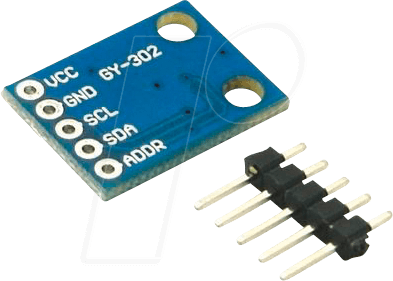
\includegraphics[width=0.5\textwidth]{assets/static/img/BH1750_pinout.jpg}
\label{fig:BH1750_pinout}

\begin{minipage}{0.5\textwidth}
\raggedright \footnotesize Fonte: Retirado de \cite{BH1750_shop} 
\end{minipage}
\end{figure}

\subsection{Sensor de Temperatura e Humidade - dht11}
\hspace*{3em}O sensor dht11, mostrado na Figura \ref{fig:dht11_pinout} é um dispositivo sensível à temperatura e humidade que pode ser utilizado em conjunto com vários microcontroladores, através do sensor capacitivo de umidade e um termistor para medir o ar e enviar um sinal no pino de saída do mesmo. O sensor dht11 possui as seguintes especificações:
\begin{enumerate}[label=\alph*)]
\itemsep0em
    \item sensor de temperatura com faixa de operação de 0ºC a 50ºC, precisão de +/- 2ºC e resolução de 1ºC;
    \item sensor de humidade com faixa de operação de 20\%HR a 90\%HR, precisão de +/- 5\%HR e resolução de 1\%HR.
\end{enumerate}

\begin{figure}[H]
\centering
\caption{Pinos dht11}
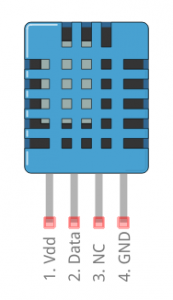
\includegraphics[width=0.3\textwidth]{assets/static/img/dht11_pinout.jpg}
\label{fig:dht11_pinout}

\begin{minipage}{0.5\textwidth}
\raggedright \footnotesize Fonte: Retirado de \cite{dht11_pinout} 
\end{minipage}
\end{figure}

\hspace*{3em}A comunicação que é mais utilizada para esse dispositivo é a \emph{adhoc} dh11. 

\end{document}
